%% CHAPTER 11 INTEGRATION -- rebuilt from Maximus's "Integration Techniques" summary PDF
\providecommand{\cautionbox}[2][CAUTION]{\begin{info}[title={#1}]#2\end{info}}
\providecommand{\ddx}{\,\mathrm{d}x}
\clearpage
\inchap{Integration}
\section{Basic Integrals}
{\renewcommand{\arraystretch}{2.1}\centering\begin{tabular}{|>{\centering\arraybackslash}m{6.6cm}|>{\centering\arraybackslash}m{7.6cm}|}\hline
\textbf{Basic}&\textbf{General form} (let $a$, $b$, $k$ be constants)\\\hline
$\displaystyle \int x^{n}\ddx=\frac{x^{n+1}}{n+1}+c,\quad n\neq-1$&$\displaystyle \int(ax+b)^{n}\ddx=\frac{(ax+b)^{n+1}}{a(n+1)}+c,\quad n\neq-1$\\\hline
$\displaystyle \int\frac1x\ddx=\ln|x|+c$&$\displaystyle \int\frac{1}{ax+b}\ddx=\frac1a\ln|ax+b|+c$\\\hline
$\displaystyle \int\mathrm{e}^{x}\ddx=\mathrm{e}^{x}+c$&$\displaystyle \int\mathrm{e}^{kx}\ddx=\frac1k\mathrm{e}^{kx}+c$\\\hline
$\displaystyle \int\sin x\ddx=-\cos x+c$&$\displaystyle \int\sin kx\ddx=-\frac1k\cos kx+c$\\\hline
$\displaystyle \int\cos x\ddx=\sin x+c$&$\displaystyle \int\cos kx\ddx=\frac1k\sin kx+c$\\\hline
$\displaystyle \int\sec^{2}x\ddx=\tan x+c$&$\displaystyle \int\sec^{2}kx\ddx=\frac1k\tan kx+c$\\\hline
\end{tabular}\par}
\section{$\mathrm{f}'(x)$ Formulas}
\cdisp{\int\mathrm{f}'(x)\left[\mathrm{f}(x)\right]^{n}\ddx&=\frac{\left[\mathrm{f}(x)\right]^{n+1}}{n+1}+c,\qquad n\neq-1\\
\int\frac{\mathrm{f}'(x)}{\mathrm{f}(x)}\ddx&=\ln|\mathrm{f}(x)|+c\\
\int\mathrm{f}'(x)\,\mathrm{e}^{\mathrm{f}(x)}\ddx&=\mathrm{e}^{\mathrm{f}(x)}+c}
\section{New Trigonometric Integrals}
\begin{itemize}
\item To find $\displaystyle\int\tan x\ddx$, $\displaystyle\int\sec x\ddx$, $\displaystyle\int\operatorname{cosec}x\ddx$, $\displaystyle\int\cot x\ddx$ --- see the \textbf{MF27}.
\item To find $\displaystyle\int\sin^{2}x\ddx$ or $\displaystyle\int\cos^{2}x\ddx$, use the \textbf{double angle formula} for $\cos2\theta$.\newline
To find $\displaystyle\int\tan^{2}x\ddx$, use the identity $\tan^{2}x=\sec^{2}x-1$.
\item The differentiation formulas for $\sec x$ and $\operatorname{cosec}x$ in the MF27 can also be used as \textbf{integration} formulas. In particular, the missing formula yields
\cdisp{\int\operatorname{cosec}^{2}x\ddx=-\cot x+c.}
\end{itemize}
\section{Standard MF27 Formulas}
{\renewcommand{\arraystretch}{2.4}\centering\begin{tabular}{|>{\centering\arraybackslash}m{6.6cm}|>{\centering\arraybackslash}m{7.6cm}|}\hline
\textbf{Standard}&\textbf{General form}\\\hline
$\displaystyle \int\frac{1}{a^{2}+x^{2}}\ddx=\frac1a\tan^{-1}\frac xa+c$&$\displaystyle \int\frac{\mathrm{f}'(x)}{a^{2}+\left[\mathrm{f}(x)\right]^{2}}\ddx=\frac1a\tan^{-1}\frac{\mathrm{f}(x)}{a}+c$\\\hline
$\displaystyle \int\frac{1}{\sqrt{a^{2}-x^{2}}}\ddx=\sin^{-1}\frac xa+c$&$\displaystyle \int\frac{\mathrm{f}'(x)}{\sqrt{a^{2}-\left[\mathrm{f}(x)\right]^{2}}}\ddx=\sin^{-1}\frac{\mathrm{f}(x)}{a}+c$\\\hline
$\displaystyle \int\frac{1}{x^{2}-a^{2}}\ddx=\frac{1}{2a}\ln\left|\frac{x-a}{x+a}\right|+c$&$\displaystyle \int\frac{\mathrm{f}'(x)}{\left[\mathrm{f}(x)\right]^{2}-a^{2}}\ddx=\frac{1}{2a}\ln\left|\frac{\mathrm{f}(x)-a}{\mathrm{f}(x)+a}\right|+c$\\\hline
$\displaystyle \int\frac{1}{a^{2}-x^{2}}\ddx=\frac{1}{2a}\ln\left|\frac{a+x}{a-x}\right|+c$&$\displaystyle \int\frac{\mathrm{f}'(x)}{a^{2}-\left[\mathrm{f}(x)\right]^{2}}\ddx=\frac{1}{2a}\ln\left|\frac{a+\mathrm{f}(x)}{a-\mathrm{f}(x)}\right|+c$\\\hline
\end{tabular}\par}
\cautionbox[IMPORTANT]{$a$ must be a (positive) \textbf{constant}.}
\begin{info}[title=Important Remark]
When using these formulas, it is \textbf{VERY COMMON} to have to complete the square first.
\end{info}
\begin{info}[title=Remark]
These formulas are commonly used together with $\mathrm{f}'(x)$ formulas to integrate \textbf{rational functions}.
\end{info}
\exlab
\cdisp{\int\frac{4x}{\sqrt{4x-x^{2}}}\ddx&=\int\frac{-2(-2x+4)+8}{\sqrt{4x-x^{2}}}\ddx\\
&=-2\int(-2x+4)\left(4x-x^{2}\right)^{-\frac12}\ddx+8\int\frac{1}{\sqrt{4-(x-2)^{2}}}\ddx\\
&=-2\cdot\frac{\left(4x-x^{2}\right)^{\frac12}}{\left(\frac12\right)}+8\sin^{-1}\frac{x-2}{2}+c\\
&=-4\sqrt{4x-x^{2}}+8\sin^{-1}\frac{x-2}{2}+c}
\clearpage
\section{Integration by Parts (IKID)}
\begin{center}\textbf{\color{red}I}\textbf{ntegrate}\quad\textbf{\color{red}K}\textbf{eep}\quad\textbf{\color{red}I}\textbf{ntegrate}\quad\textbf{\color{red}D}\textbf{ifferentiate}\end{center}
\cdisp{IK-\int ID\ddx}
\exlab
\cdisp{\int\underbrace{x}_{\text{K/D}}\,\underbrace{\mathrm{e}^{x}}_{\text{I}}\ddx=\underbrace{\mathrm{e}^{x}}_{\text{I}}\,\underbrace{x}_{\text{K}}-\int\underbrace{\mathrm{e}^{x}}_{\text{I}}\,\underbrace{1}_{\text{D}}\ddx}
\begin{itemize}
\item It is possible to make the \textbf{wrong choice} of which expression to integrate. In such scenarios, the $\int ID\ddx$ will look \textit{worse} than the original problem.
\item It is common to have to \textbf{IKID twice}. Consider this approach if you are unable to continue.
\end{itemize}
\cautionbox[IMPORTANT]{Integration by parts is often used as the \textbf{last resort}, i.e.\ please consider \textbf{ALL OTHER INTEGRATION TECHNIQUES} first.}
\textbf{Common tricks}
\begin{itemize}
\item \textbf{IKID by multiplying by 1.}
\cdisp{\int\ln x\ddx=\int1\cdot\ln x\ddx=\dots}
\item \textbf{Non-obvious splitting.}
\cdisp{\int x^{3}\mathrm{e}^{x^{2}}\ddx=\int x^{2}\cdot x\mathrm{e}^{x^{2}}\ddx=\dots}
Here, we can integrate $x\mathrm{e}^{x^{2}}$ using the $\int\mathrm{f}'(x)\mathrm{e}^{\mathrm{f}(x)}\ddx$ formula.
\item \textbf{Loop method.}
\cdisp{\int\mathrm{e}^{x}\cos x\ddx&=\mathrm{e}^{x}\cos x+\int\mathrm{e}^{x}\sin x\ddx\\
&=\mathrm{e}^{x}\cos x+\mathrm{e}^{x}\sin x-\int\mathrm{e}^{x}\cos x\ddx}
Therefore,
\cdisp{2\int\mathrm{e}^{x}\cos x\ddx&=\mathrm{e}^{x}\cos x+\mathrm{e}^{x}\sin x+c\\
\int\mathrm{e}^{x}\cos x\ddx&=\frac12\left(\mathrm{e}^{x}\cos x+\mathrm{e}^{x}\sin x\right)+c}
\end{itemize}
\clearpage
\section{Integration by Substitution}
Given $\displaystyle\int\mathrm{f}(x)\ddx$ and a substitution $u=\dots$, apply:\par
\textbf{Step 1:} Substitute $u$ into $\mathrm{f}(x)$.\par
\textbf{Step 2:} Find $\dfrac{\mathrm{d}x}{\mathrm{d}u}$, and substitute it into the integral.\par
\textbf{Step 3:} \textit{(Only for definite integrals)} Substitute the limits of integration from $x$ values to $u$ values.\par
{\setlength{\columnseprule}{0.4pt}\begin{multicols}{2}
{\centering\textbf{Indefinite Integral}\par}
\exlab
\fhlp{Using the substitution $x=\sin u$, where $0\leqslant u\leqslant\frac{\pi}{2}$, find $\displaystyle\int\sqrt{1-x^{2}}\ddx$.}\par
\cdisp{&\int\sqrt{1-x^{2}}\ddx,\qquad x=\sin u\\
={}&\int\underbrace{\sqrt{1-\sin^{2}u}}_{\text{Step 1}}\,\underbrace{\cos u\,\mathrm{d}u}_{\text{Step 2}}\\
={}&\int\sqrt{\cos^{2}u}\,\cos u\,\mathrm{d}u\\
={}&\int\cos^{2}u\,\mathrm{d}u\\
={}&\frac12\int\left(1+\cos2u\right)\mathrm{d}u\\
={}&\frac12\left(u+\frac12\sin2u\right)+c\\
={}&\frac12u+\frac12\sin u\cos u+c\\
={}&\frac12\sin^{-1}x+\frac12x\sqrt{1-x^{2}}+c}
\begin{center}\fbox{\begin{minipage}{5.4cm}\centering\vspace{1mm}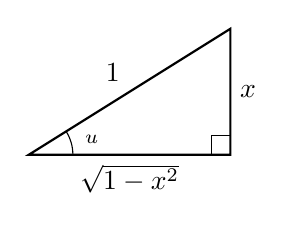
\begin{tikzpicture}[scale=1.6]
\draw[thick] (0,0)--(1.6,0)--(1.6,1)--cycle;
\draw (1.45,0)--(1.45,0.15)--(1.6,0.15);
\node[above left] at (0.8,0.5){$1$}; \node[right] at (1.6,0.5){$x$}; \node[below] at (0.8,0){$\sqrt{1-x^{2}}$};
\draw (0.35,0) arc(0:32:0.35); \node at (0.5,0.12){\scriptsize$u$};
\end{tikzpicture}\par
\cdisp{\sin u&=x\\\cos u&=\sqrt{1-x^{2}}}\end{minipage}}\end{center}
\columnbreak
{\centering\textbf{Definite Integral}\par}
\exlab
\fhlp{Using the substitution $x=\sin u$, find the exact value of $\displaystyle\int_{0}^{\frac12}\sqrt{1-x^{2}}\ddx$.}\par
\cdisp{&\int_{0}^{\frac12}\sqrt{1-x^{2}}\ddx,\qquad x=\sin u\\
x=0\ &\Rightarrow\ u=0\\
x=\frac12\ &\Rightarrow\ u=\frac{\pi}{6}\\
\int_{0}^{\frac12}\sqrt{1-x^{2}}\ddx&=\int_{0}^{\frac{\pi}{6}}\sqrt{1-\sin^{2}u}\,\cos u\,\mathrm{d}u\\
&=\int_{0}^{\frac{\pi}{6}}\cos^{2}u\,\mathrm{d}u\\
&=\frac12\int_{0}^{\frac{\pi}{6}}\left(1+\cos2u\right)\mathrm{d}u\\
&=\frac12\left[u+\frac12\sin2u\right]_{0}^{\frac{\pi}{6}}\\
&=\frac12\left[\left(\frac{\pi}{6}+\frac12\sin\frac{\pi}{3}\right)-\left(0+\frac12\sin0\right)\right]\\
&=\frac12\left(\frac{\pi}{6}+\frac{\sqrt3}{4}\right)\\
&=\frac{\pi}{12}+\frac{\sqrt3}{8}}
\end{multicols}}
\begin{info}[title=Remark]
Remember to sub the final answer back to be in terms of $x$, unless it's a \textbf{definite integral}.
\end{info}
